\chapter{Analysis of Stitched Image}

\section{About}
Analysis on the stitched image formed from previous steps is an important part of the system. This analysis helps to derive useful insights from the image which is used to provide prescription to the farmers.
This chapter describes the usgae of analysis techniques like Vegetation Indices as a measure of crop health combined with machine learning algorithms for better prediction. Classification of images taken by the farmer, with the use of deep learning is also dicussed. 
 
\section{Comparison of Different Image Analysis Techniques}
Given a framework that gathers the necessary data, the decision making to be performed requires knowledge extraction from these data. Hyperspectral images contain a lot of useful information that can be analyzed to generate many insightful results. These results can then help to produce a reliable prescription map and present the solutions in a way that can be understood by the farmers.

Over the years, a number of Vegetation Indices (VIs) have been developed by combining two or more wavebands in the hyperspectral images in ratios and/or differences, to highlight various crop conditions. However, one of the problems in applying VIs to crop yield estimation is the difficulty in choosing the most appropriate vegetation index in a specific situation (Barrett and Curtis 1999). In fact, various environmental factors, such as background effects and crop canopy conditions, have been shown to be potential sources of noise, which affect the spectral reflectance in canopy level (Aparicio et al., 2000). Ironically, these difficulties, to identify the most useful wavelengths or VIs under specific environmental conditions, have been heightened with the recent proliferation of large volume of data available from hyperspectral and broadband sensors. Sensitivity of vegetation indices and tapping the full potential of large quantities of spectral information acquired with the latest sensors are currently the most important impediments to successfully applying remote sensing technologies to precision farming.

Artificial intelligence and especially machine learning have contributed to the creation of control systems in agriculture. Machine learning is the process of discovering previously unknown and potentially useful information from data. It is one of the most important and useful data mining tools that can discover unknown regularities and patterns from data sets. There are a lot of machine learning algorithms like Support Vector Machines(SVM), Simple Multivariate Linear Regressions(SMLR), Decision Trees(DT), Neural Networks(NN), etc. available that can be utilized for recognizing intricate patterns in data. Implementation of these algorithms in agricultural domain have shown inspiring results as shown in Table ~\ref{tab: tab1}.
 
\begin{figure}[t]
	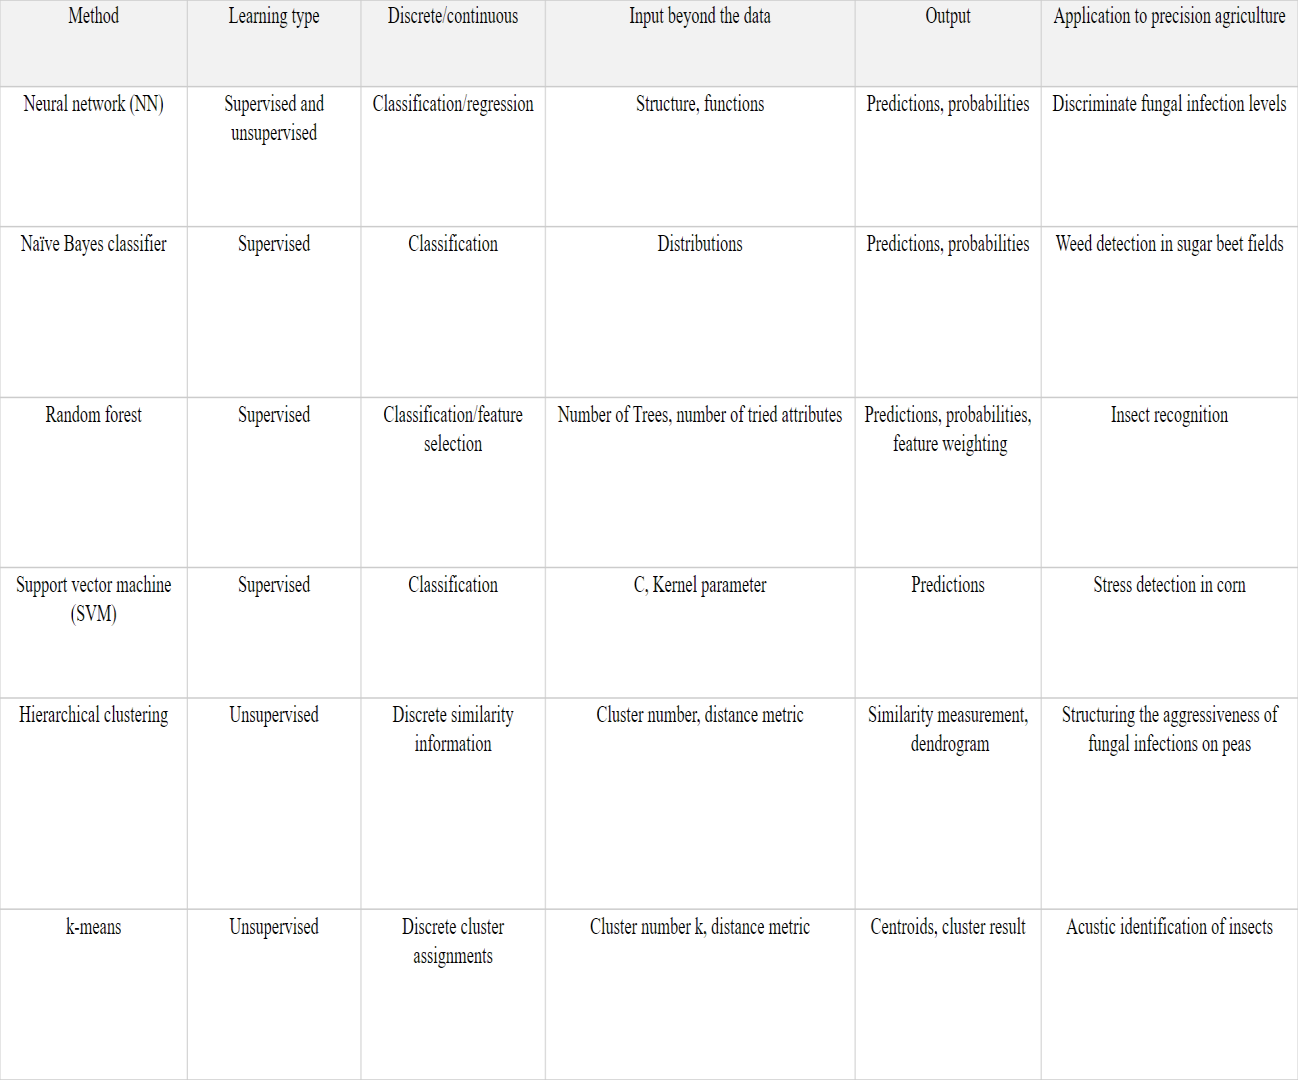
\includegraphics[width=1\linewidth]{extra-9}
	\centering
\captionof{table}{Comparison between different machine learning algorithms along with their application in agricultural domains} \label{tab: tab1}
\end{figure}

Deep Neural Networks (DNNs), have generated a strong interest in their potential effectiveness in estimating various field and crop conditions. The ability of DNNs to associate complicated information with target attributes without any constraints for sample distribution, make them ideal for describing the intricate and complex non-linear relationships which exist between canopy-level spectral signatures and various crop condition. In fact, successful applications have already been reported for surface water quality assessment, soil moisture estimation, biomass estimation, and yield prediction. A Deep Neural Network (DNN) is a computational model which mimics the human nervous system and decision-making process. Although some technical difficulties, such as the low interpretability of the developed models, the complexity involved in optimizing the model structure, and the high processing power required for the training process, once made the intensive application of this techniques difficult, recent improvements in computing power and learning algorithms has increased the applicability of the method in various fields.

A combination of VI methods, mainly Normalized Differnce Vegetation Index(NDVI) and machine learning is used as a part of analysis on hyperspectral data. This requires a lot of labelled dataset but due to its unavailablity we needed to generate our own data. Figure~\ref{fig: dada} shows the flow of the algorithm as used by us to generate labellled data and train the SoftMax model. NDVI calculations are done on the stitched image whose output is then fed into the K-means clustering algorithm to generate labelled data. This labelled data is then used to train the SofMax regression model. 
\begin{figure}[h]
	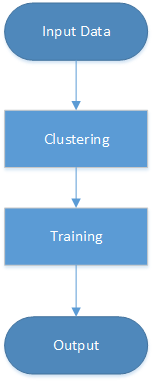
\includegraphics[height=1.0\linewidth]{dada}
	\centering
	\caption{\label{fig: dada}Flowchart to generate labelled data and train machine learning model}
\end{figure}


Evaluation of a new stitched image of the farm is done using this SoftMax model to determine critical areas on the farm which are shown by different colors on the output image which is overlaid on Google Map. Once the critical areas are determined we can go a step ahead to analyse the problem in those areas on the farm. The widespread distribution of smartphones among crop growers around the world with an expected 5 billion smartphones by 2020 offers the potential of turning the smartphone into a valuable tool for diverse communities growing food. To derive the potential of this fact along with the abilities of deep learning, we trained a deep learning model to recognize diseases in crops. The farmer can go to the critical areas on the farm and take a photograph of infected crops which will be evaluated against our deep learning model to provide a prescription.



\section{Image Analysis Using Indexing}

The hyperspectral images we have carry vital information that can be analyzed to deduce important parameters about crops. VI based methods provide many ways to explore this using specific algorithms designed to perform analysis on such images. Some of those which we wish to use are Normalized Difference Vegetation Index (NDVI), to know the chlorophyll content in leaves. A flowchart of the process is shown in Fig.~\ref{fig: extra-10}.

\begin{figure}[h]
	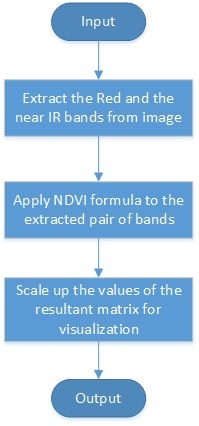
\includegraphics[height=0.9\linewidth]{extra-10}
	\centering
	\caption{\label{fig: extra-10}Image analysis using VI based methods}
\end{figure}


\subsection{Normalized Difference Vegetation Index}

The Normalized Difference Vegetation Index (NDVI) is a numerical indicator that uses the visible and near-infrared bands of the spectrum, and is adopted to analyze remote sensing measurements and assess whether the target being discovered contains live inexperienced vegetation or not. NDVI has found a wide application in vegetative studies because it has been accustomed estimate crop yields, pasture performance, and rangeland carrying capacities among others. It is often directly associated with different ground parameters like percentage of ground cowl, photosynthetic activity of the plant, surface water, leaf  area index and the quantity of biomass. NDVI was first used in 1973 by Rouse et al. from the Remote Sensing Centre of Texas A$\&$M University.

Generally, healthy vegetation will absorb most of the visible lightweight that falls on that, and reflects a large portion of the near-infrared lightweight. Unhealthy or sparse vegetation reflects additional visible lightweight and fewer near-infrared lightweight. Bare soils on the different hand mirror moderately in each the red and infrared portion of the spectrum. Since we recognize the behavior of plants across the spectrum, we will derive NDVI info by specializing in the satellite bands that area unit most sensitive to  vegetation info (near-infrared and red). The bigger the distinction so between the near-infrared and therefore the red coefficient, the more vegetation there has to be. The NDVI algorithm subtracts the red reflectance values from the near-infrared and divides it by the sum of near-infrared and red bands.

\begin{equation} \label{eq: eq-1}
NDVI = (NIR-RED)/(NIR+RED)
\end{equation}
This formulation allows us to cope with the fact that two identical patches of vegetation could have different values if one were, for example in bright sunshine, and another under a cloudy sky. The bright pixels would all have larger values, and therefore a larger absolute difference between the bands. This is avoided by dividing by the sum of the reflectance. 

\begin{figure}[h]
	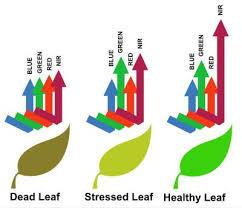
\includegraphics[height=0.5\linewidth]{fin_img_8}
	\centering
	\caption{\label{fig: reflectance}Reflectances from different types of leaves}
\end{figure}

Theoretically, NDVI values are represented as a ratio ranging in value from -1 to 1 but in practice extreme negative values represent water, values around zero represent bare soil and values over 0.6 represent dense green vegetation. Reflectances from different types of leaves is shown in Fig.~\ref{fig: reflectance}.


\subsection{Clustering and Classification}
After all the index calculations are done we are left with areas with different discrete patches that may have the same index range. The next step would be to cluster the similar data (pixel values) into a single color coded areas. The clustering is done using K-means algorithm. This clustered information is then used to train a SoftMax regression model for classification of new images as mentioned previously.

\subsubsection{K-means Algorithm}
K-means is one of the best unsupervised learning algorithms that solve the well-known bunch downside. Initially number of centers, which is k, is decided according to the Elbow Rule which minimizes the cost function with an appropriate number of clusters. The main idea is to outline kcenters, one for each cluster. These centers should be placed in a crafty method attributable to totally different location causes different result. So, the better selection is to put them the maximum amount as potential secluded from one another.

The next step is to assign the closest center to each data point. At this point we'd like to recalculate k new centroids as center of mass of the clusters ensuing from the previous step. After we have a tendency to have these k new centroids, a new binding must be done between constant data set points and therefore the nearest new center. A loop has been generated. As a result of this loop we could notice that the k centers amendment their location step by step till no additional changes square measure done or in different words centers don't move from now on. Finally, this algorithm aims at minimizing associate objective operate is aware of as square error operate given by:


\begin{equation} \label{eq: eq-3}
J(V) = \sum_{i=1}^{C}\sum_{j=1}^{C_i} (\begin{Vmatrix}x_i-v_i
\end{Vmatrix})^2
\end{equation}
\begin{equation*} 
\begin{Vmatrix}x_i-v_i

\end{Vmatrix} \text{is the Euclidean distance between } x_i \quad \& \quad v_j 
\end{equation*}
\begin{equation*} 
c_i \text{ is the number of data points in the $i_{}^{th}$ cluster}
\end{equation*}
\begin{equation*} 
c \text{ is the number of cluster centers}
\end{equation*}


Algorithmic steps for k-means clustering:

Let $X = \begin{Bmatrix} x_1,x_2,x_3,...,x_n \end{Bmatrix}$ be the set of data points and $V = \begin{Bmatrix} v_1,v_2,v_3,...,v_c \end{Bmatrix}$ be the set of centers.

\begin{enumerate}
	\item Randomly select ‘c’ cluster centers.
	\item Calculate the distance between each data point and cluster centers.
	\item Assign the data point to the cluster center whose distance from the cluster center is minimum of all the cluster centers.
	\item Recalculate the new cluster center using,
	\begin{equation} \label{eq: eq-4}
	v_i = (1/C_i)  \sum_{j=1}^{C_i}x_i
	\end{equation}
	where $c_i \text{ represents the number of data points in the $i_{}^{th}$ cluster}$
	\item Recalculate the distance between each data point and new obtained cluster centers.
	\item If no data point was reassigned then stop, otherwise repeat from step 3.	
\end{enumerate}


\subsection{Softmax Regression Model}
Once we have  labelled data we can train a machine learning model for better analysis of the farm. In our case we employ the use of SoftMax regression model to learn the range of NDVI values. Softmax regression is a generalization of logistic regression to the case where we want to handle multiple classes. It is a regression model which generalizes the logistic regression to classification problems where the output can take more than two possible values. SoftMax regression is competitive in terms of CPU and memory consumption. The Softmax Regression is preferred when we have features of different type (continuous, discrete, dummy variables etc), nevertheless given that it is a regression model, it is more vulnerable to multicollinearity problems and thus it should be avoided when our features are highly correlated. The structural architecture of the algorithm is shown in Fig.~\ref{fig: softmax}.
\begin{figure}[t]
	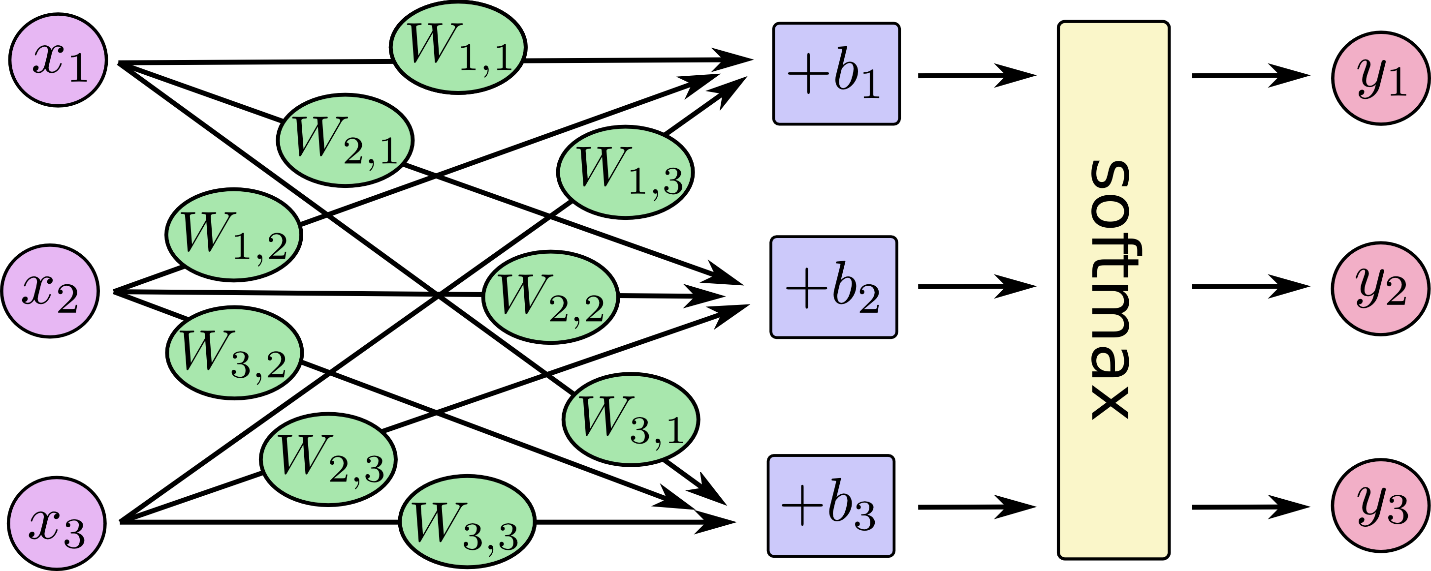
\includegraphics[width=1.0\linewidth]{fin_img_11}
	\centering
	\caption{\label{fig: softmax}Basic structure of Softmax Model}
\end{figure}

This model divides the input farm image into different color coded regions depending upon the NDVI values.This image is then overlayed onto the Google Map for better visualization of the farm. This image shows critical areas on the farm which can further be analysed for crop disease prediction using deep learning.


